\section{Convolution} 

  Convolutional networks work with images, so let's introduce a nice way to represent them as vectors. 

  \begin{definition}[Image]
    An image is a vector in some tensor product space. More specifically, avoiding the technicality that each pixel element is bounded and discrete, 

    \begin{enumerate}
      \item A \textbf{grayscale image} of resolution of $H \times W$ is a vector in $\mathbb{R}^{H} \otimes \mathbb{R}^{W}$. 
      \item An \textbf{image} with $C$ channels of the same resolution is an element of $\mathbb{R}^{C} \otimes \mathbb{R}^H \otimes \mathbb{R}^W$. 
      \item A \textbf{video} with $C$ channels and of the same resolution is an element of $\mathbb{R}^T \otimes \mathbb{R}^C \otimes \mathbb{R}^H \otimes \mathbb{R}^W$, where $T$ is the time dimension which is usually represented in some discrete frames.
    \end{enumerate} 
    Usually, we denote the height/width as the \textbf{spatial dimension}, the colors and the \textbf{channel dimension}, and time as the \textbf{temporal dimension}.\footnote{Everything we talked about so far applies to images when treated as vectors. In fact, so far we have been interpreting images of size $(C, H, W)$ through the isomorphism $\phi: \mathbb{R}^{C} \otimes \mathbb{R}^H \otimes \mathbb{R}^W \rightarrow \mathbb{R}^{C \times H \times W}$ that essentially ``unravels" the image. }
  \end{definition}

  Note that the terminology above is general convention, and tensors of arbitrary shape may exist that encode---say time over two dimensions. So far, we have seen the power of multilayer perceptrons and their predictive ability on moderately sized vectors. In fact, if we process the MNIST with a simple MLP of 2 layers and 512 nodes each, we can easily get $95\%$ accuracy within 10 epochs. However, these MNIST pictures are extremely low resolution, at $1 \times 28 \times 28$, and for even moderately sized images we can that there is a huge blowup of parameters needed. \footnote{For example, an RGB image that is $3 \times 1024 \times 1024$ would have ~3m parameters, and then defining a dense linear map to even 1000 dimensions would take 3 billion parameters. Given that 32-bit floating point is $4$ bytes, this already takes up 12GB of memory just to load the network.} Clearly, this is not efficient, and so the only way to move on is to create a sparser representation of the network. Therefore, can we create a sparser representation of a linear map that does sacrifice too much expressibility for memory? With convolutional kernels\footnote{Note that this is completely different than the kernels mentioned in supervised learning, with support vector machines and RKHS.}, the answer is yes. In 1994, Yann LeCunn and Yoshua Bengio in Bell Labs published \cite{cnn} which introduced the \textit{convolutional neural network}. 

  The only layer know is a fully-connected layer. Now we will learn about our second type of layer. 

  \begin{definition}[1D Convolutional Layer]
    A \textbf{1D convolutional operator/layer} of 
    \begin{enumerate}
      \item input channels $C_{\mathrm{in}}$ 
      \item output channels $C_{\mathrm{out}}$ 
      \item kernel size $K$ 
      \item stride $S$
    \end{enumerate}
    is an operator $\phi: \mathbb{R}^{C_{\mathrm{in}}} \times \mathbb{R}^L \rightarrow \mathbb{R}^{C_{\mathrm{out}}} \times \mathbb{R}^{L_{\mathrm{out}}}$, where $C$ is the channel dimension and $L$ is the spatial dimension. We can view 
    \begin{equation}
      \phi(x)_{c, i} = \sum_{} 
    \end{equation}
  \end{definition}

  \begin{definition}[2D Convolutional Layer]
    A \textbf{convolutional operator/layer} of 
    \begin{enumerate}
      \item size 
    \end{enumerate}
  \end{definition}

  \begin{definition}[3D Convolutional Layer]
    A \textbf{convolutional operator/layer} of 
    \begin{enumerate}
      \item size 
    \end{enumerate}
  \end{definition}

  \begin{figure}[H]
    \centering 
    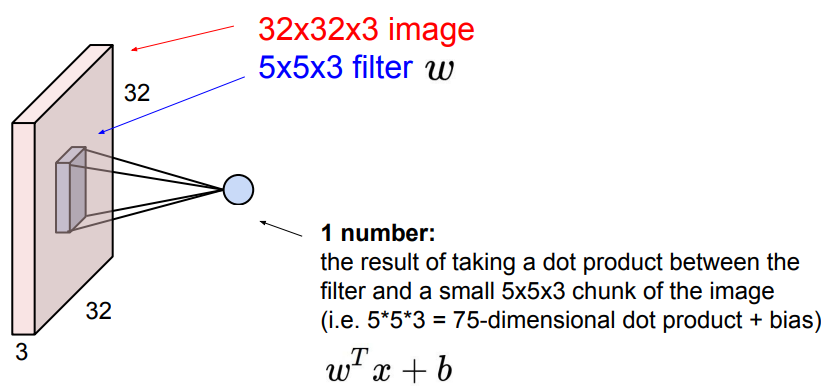
\includegraphics[scale=0.35]{img/kernel1.png}
    \caption{} 
    \label{fig:kernel1}
  \end{figure}

  \begin{figure}[H]
    \centering 
    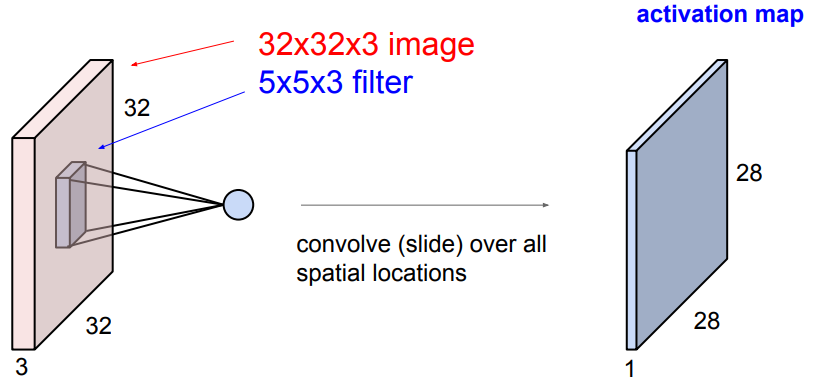
\includegraphics[scale=0.35]{img/kernel2.png}
    \caption{} 
    \label{fig:kernel2}
  \end{figure}

  \begin{figure}[H]
    \centering 
    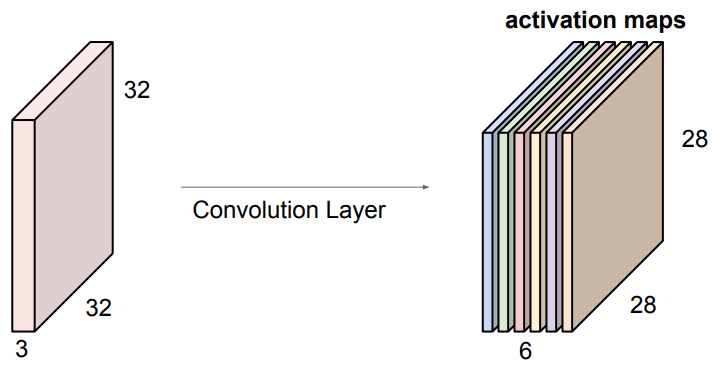
\includegraphics[scale=0.35]{img/kernel3.png}
    \caption{} 
    \label{fig:kernel3}
  \end{figure}

  \begin{definition}[Convolutional Kernel]
    A \textbf{convolution operator} on a vector space $V$ representing an image space is simply a special type of linear map that is parameterized by a much smaller set of numbers, stored within a \textbf{kernel} or \textbf{filter}. In all honesty, it is much easier to go through examples to see how they work, so in this definition I will focus more on describing the hyperparameters. Given an image of shape $(C, H, W)$, the convolution is essentially a sliding window that computes a dot product between the kernel and the window that the kernel covers over the image. 
    \begin{enumerate}
      \item The sliding window size is $(W_{ker}, H_{ker})$, which is conventionally square but does not need to be. 

      \item This sliding window must compute over all channels, so in fact it is of shape $(C_{in}, W_{ker}, H_{ker})$. This would generate one output channel image. 

      \item Multiple kernels can be used concurrently to generate different channel images. Therefore, if we want to have a collection of $C_{\text{out}}$ outputs that are extracted from each kernel, our total kernel would be a collection of $C_{out}$ kernels of shape $(C_{in}, W_{ker}, H_{ker}, C_{out})$. Therefore, the total equation is 
      \begin{equation}
        (X \ast K)_{f, i, j} \coloneqq \sum_c \sum_{p, q} X_{c, i + p, j + q} \cdot K_{c, p, q, f} + b_{f, i, j}
      \end{equation}

      where $c$ is the channel index, $p, q$ are the location indices, $f$ is the output channel index, and $b$ is some bias term. 

      \item The stride parameter $s$ can also be set to determine the stride of the kernel $\mathcal{K}$. 

      \item Another thing to note is that the output image of a kernel would be slightly smaller than the input image, since the kernel cannot go over the edge. However, there are padding schemes to preserve the original dimensions. 
    \end{enumerate}
    From the equation above, we can see that a convolutional layer, assuming that it has full padding, is a linear map  
    \begin{equation}
      \mathcal{K} : \mathbb{R}^{C_{in}} \otimes \mathbb{R}^H \otimes \mathbb{R}^W \rightarrow \mathbb{R}^{C_{out}} \otimes \mathbb{R}^H \otimes \mathbb{R}^W
      \label{eq:conv_mapping}
    \end{equation}
    The vector space of linear maps mapping between these two spaces has $C_{in} H^2 W^2 C_{out}$ dimensions, which is extremely large, but parameterizing $\mathcal{K}$ with this matrix reduces the set of relevant convolutional maps to a subspace that is $(1 + C_{in} H_{ker} W_{ker}) C_{out}$ dimensional (with the $+1$ due to a bias term, making this an affine map). This is essentially what a convolution is: sparse matrix multiplication, and there is nothing else that makes it different from a classical feedforward neural network. It's just computationally efficient matrix multiplication for high-dimensional vectors. 
  \end{definition}

  In addition to computational efficiency and weight sharing, convolutional operators capitalize on the principle of \textbf{locality}, i.e. that pixels are directly related to adjacent pixels. For example, a pixel representing a portion of a dog's ear would not be related to the background, but the color and positioning should be related to the dog's face, which may be within a certain neighborhood around. This has been shown to be similar to the human visual system and is thus well motivated. 

  Though this next topic has more to do with classical image processing than computer vision, there are a surprising number of features that these convolutional filters can extract from an image. By treating them as a discretized form of a partial derivative (as the vertical and horizontal edge detection) or as the Hessian operator (sharpening), we can extract many features from them.  

  \begin{example}[Blurs, Edge Detection]
    Given the original image below, we show various convolutional filters applied on the image. Note that the kernel matrix may have the property that all of its entries sum to $1$, meaning that on average, the expected value of the brightness of each pixel will be $0$, and the values will be left unchanged on average. However, this is not a requirement.  
    \begin{align*}
      \mathrm{Original} = \begin{bmatrix} 1 & 0 & 0 & 0 & 0 \\ 0 & 1 & 0 & 0 & 0 \\ 0 & 0 & 1 & 0 & 0 \\ 0 & 0 & 0 & 1 & 0 \\ 0 & 0 & 0 & 0 & 1 \end{bmatrix} & 
      \mathrm{Mean} = \frac{1}{25} \begin{bmatrix} 1 & 1 & 1 & 1 & 1 \\ 1 & 1 & 1 & 1 & 1 \\ 1 & 1 & 1 & 1 & 1 \\ 1 & 1 & 1 & 1 & 1 \\ 1 & 1 & 1 & 1 & 1 \end{bmatrix} & 
      \mathrm{Gaussian} = \frac{1}{273} \begin{bmatrix} 1 & 4 & 7 & 4 & 1 \\ 4 & 16 & 26 & 16 & 4 \\ 7 & 26 & 41 & 26 & 7 \\ 4 & 16 & 26 & 16 & 4 \\ 1 & 4 & 7 & 4 & 1 \end{bmatrix} \\   
      \mathrm{Sharpen} = \begin{bmatrix} 0 & -1 & 0 \\ -1 & 5 & -1 \\ 0 & -1 & 0 \end{bmatrix} & 
      \mathrm{Horizontal} = \begin{bmatrix} -1 & 0 & 1 \\ -2 & 0 & 2 \\ -1 & 0 & 1 \end{bmatrix} & 
      \mathrm{Vertical} = \begin{bmatrix} -1 & -2 & -1 \\ 0 & 0 & 0 \\ 1 & 2 & 1 \end{bmatrix} 
    \end{align*}

    These filters visually output the following images. Note that these filters are each acting on the image by acting individually on each channel and then combining the 3 outputs to create the new RGB image. 
    \begin{figure}[H]
      \centering
      \begin{subfigure}[b]{0.32\textwidth}
      \centering
          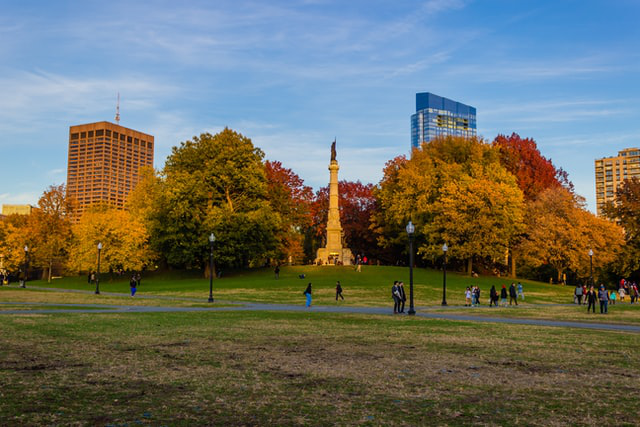
\includegraphics[width=\textwidth]{img/Park_Full.png}
          \caption{Original image. }
          \label{fig:original_image}
      \end{subfigure}
      \begin{subfigure}[b]{0.32\textwidth}
      \centering
          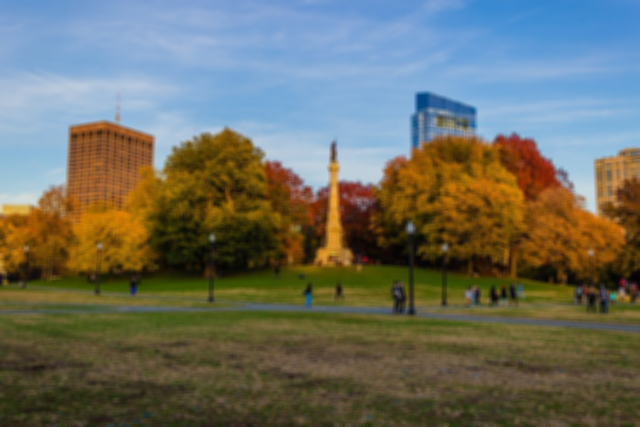
\includegraphics[width=\textwidth]{img/Mean_Blur.png}
          \caption{$5 \times 5$ mean blur applied. }
          \label{fig:mean_blur_image}
      \end{subfigure}
      \begin{subfigure}[b]{0.32\textwidth}
      \centering
          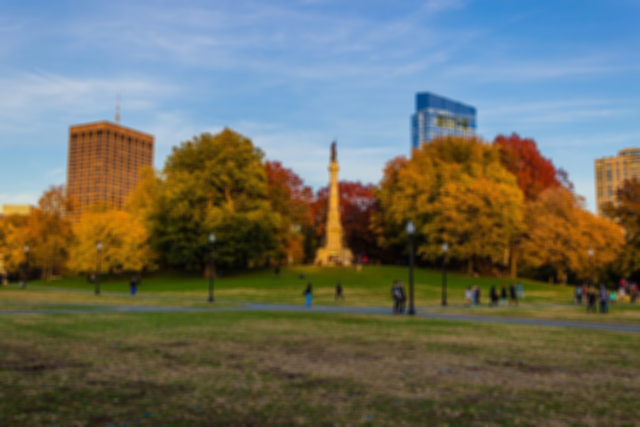
\includegraphics[width=\textwidth]{img/Gaussian_Blur.png}
          \caption{$5 \times 5$ Gaussian blur applied. }
          \label{fig:normal_blur_image}
      \end{subfigure}
      
      \begin{subfigure}[b]{0.32\textwidth}
      \centering
          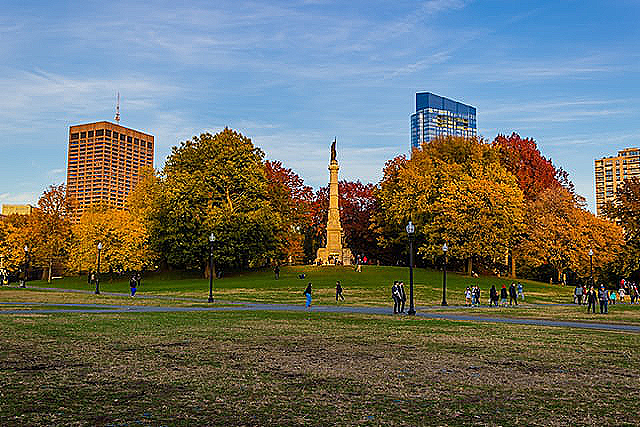
\includegraphics[width=\textwidth]{img/Sharpen.png}
          \caption{Sharpening kernel. } \label{fig:sharpened_image}
      \end{subfigure} 
      \begin{subfigure}[b]{0.32\textwidth}
      \centering
          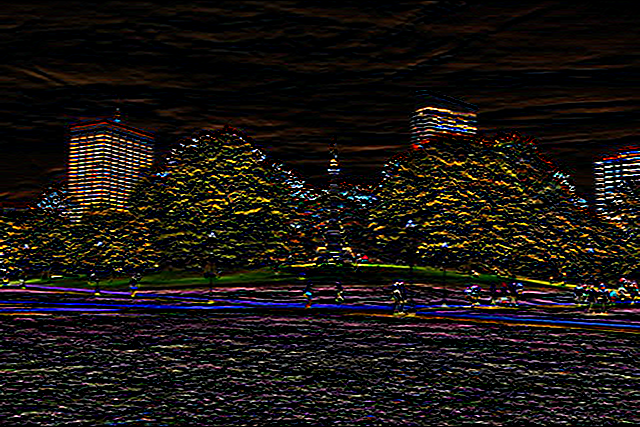
\includegraphics[width=\textwidth]{img/Horizontal.png}
          \caption{Horizontal edge detection. }
          \label{fig:horizontal_edge}
      \end{subfigure}
      \begin{subfigure}[b]{0.32\textwidth}
      \centering
          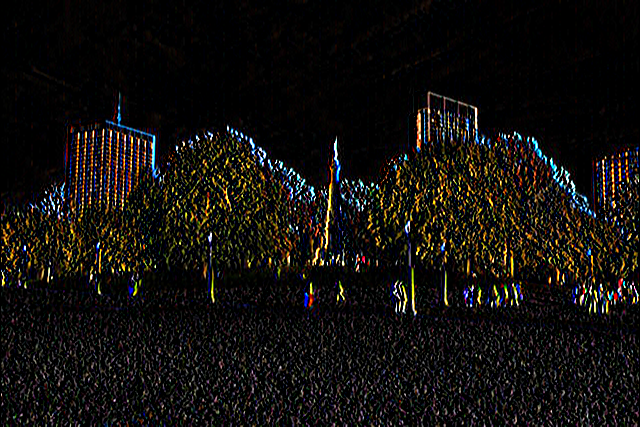
\includegraphics[width=\textwidth]{img/Vertical.png}
          \caption{Vertial edge detection. }
          \label{fig:vertical_edge}
      \end{subfigure} 

      \caption{Different convolutional kernels acting on the same image. Several useful features like edges can be detected with these simple linear maps. }
      \label{fig:feature_extraction}
    \end{figure}
  \end{example}

  We have seen in the example above that we can interpret each output channel of a convolution as a feature. That is, our original input image with $C_{in} = 3$ channels may go through a convolution that has $C_{out} = 10$ output channels, producing $10$ grayscale images. Each of these images may represent a feature that is extracted from the image through a custom kernel. When we stack convolutional layers together (with nonlinearities in between, of course), we can produce more complicated transformations that extract more abstract features. For example, while the first layer or two may extract certain edges within a dog, perhaps the fourth or fifth convolutional layer will be able to detect the presence of ears. This is a hand-wavy example, but if you actually visualize the outputs of these layers during forward prop, it is possible to see this in action.  

